\documentclass{sigchi}

% --- Copyright notice ---
\clubpenalty=10000 
\widowpenalty = 10000

% To make various LaTeX processors do the right thing with page size.
\def\pprw{8.5in}
\def\pprh{11in}
\special{papersize=\pprw,\pprh}
\setlength{\paperwidth}{\pprw}
\setlength{\paperheight}{\pprh}
\setlength{\pdfpagewidth}{\pprw}
\setlength{\pdfpageheight}{\pprh}

% create a shortcut to typeset table headings
\newcommand\tabhead[1]{\small\textbf{#1}}

\usepackage{balance}
\usepackage{times}
\usepackage{url}
\usepackage{graphicx} % for EPS use the graphics package instead
%\usepackage{bibspacing} % save vertical space in references
\usepackage{subcaption}

%\pagenumbering{arabic} % - remove for final camera-ready
\pagenumbering{gobble}

\makeatletter
\def\url@leostyle{%
  \@ifundefined{selectfont}{\def\UrlFont{\sf}}{\def\UrlFont{\small\bf\ttfamily}}}
\makeatother
\urlstyle{leo}

% Make sure hyperref comes last of your loaded packages, 
% to give it a fighting chance of not being over-written, 
% since its job is to redefine many LaTeX commands.
\usepackage[pdftex]{hyperref}
\hypersetup{
pdftitle={Support Support : Visualizing Part Orientation and Effects Thereof for 3D Printing},
pdfauthor={Valkyrie Savage & Derrick Cheng},
pdfkeywords={3D printing, prototyping, fabrication},
bookmarksnumbered,
pdfstartview={FitH},
colorlinks,
citecolor=black,
filecolor=black,
linkcolor=black,
urlcolor=black,
breaklinks=true,
}

\begin{document}
%use these commands while writing
\newcommand {\derrick}[1]{{\color{red}\bf{DC: #1}\normalfont}}
\newcommand {\valkyrie}[1]{{\color{blue}\bf{VS: #1}\normalfont}}

%comment out the above and uncomment these for final submit
%\newcommand {\derrick}[1]{}
%\newcommand {\valkyrie}[1]{}

\newcommand {\bt}[1]{\textbf{#1} \normalfont}
\newcommand{\squishlist}{
 \begin{list}{$\bullet$}
  { \setlength{\itemsep}{0pt}
     \setlength{\parsep}{3pt}
     \setlength{\topsep}{3pt}
     \setlength{\partopsep}{0pt}
     \setlength{\leftmargin}{1.5em}
     \setlength{\labelwidth}{1em}
     \setlength{\labelsep}{0.5em} } }
\newcommand{\squishend}{
  \end{list}  }
 %defines comments, squishlist, other macros.

\title{Support Support : Visualizing Part Orientation and Effects Thereof for 3D Printing}

%\numberofauthors{1}
%  \author{
%    \alignauthor Author(s) Removed for Blind Review Process
%  }

\numberofauthors{1}
\author{
  \alignauthor Valkyrie Savage \& Derrick Cheng\\
    \affaddr{University of California, Berkeley}\\
    \affaddr{Berkeley Institute of Design, Computer Science Division}\\
    \email{\{valkyrie,derrick\}@eecs.berkeley.edu}\\
}

\maketitle


\begin{figure*}
\centering
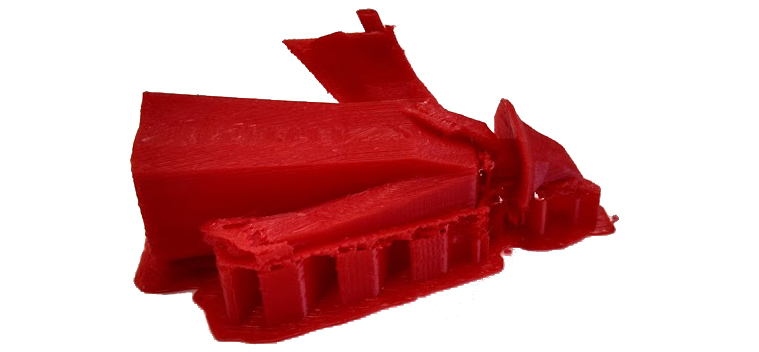
\includegraphics[width=7in]{images/printed.jpg}
\caption{A 3D print with a balance of material use, print time, and surface area covered by support.  The rough structures at the bottom are the support material, which can be difficult to remove.}
\label{fig:printed}
\end{figure*}

\begin{abstract}
3D printers proliferate, yet every step leading from idea to print is too complicated for all but dedicated users to perform.  Those creating 3D printable objects have many concerns related to how the printing will go. While very fancy printers have multiple material capabilities and easy-dissolve supports, hobbyist-level machines are typically limited to a single material used for both the model and the model supports. Thus, one common user concern is how difficult support removal will be; this is based on the angle of attachment between model and support (e.g. removing support oblique to the model is more difficult), the accessibility of the area of support material (e.g. support is easy to remove from a flat, exposed surface and more difficult to remove from a curved surface partially obscured by other faces), and the amount of support (e.g. more support takes longer). Another common concern is the total printing time; users don't necessarily want to wait for long prints. A third issue is material waste; excess support material used in a print must be thrown away and cannot be used again.  Finally, users may have areas of high detail in which they do not want to have support in their final prints, as support removal can break or damage finely-details surfaces.  Unfortunately, these four issues are often at odds, and all depend upon the model's orientation in the bed.  We have designed a tool which automatically generates several random model orientations and calculates statistics for each of these four metrics.  We present these calculations to the user in an interactive web-based tool.
\end{abstract}

\keywords{Prototyping; Fabrication; 3D Printing}

\category{H.5.2}{User Interfaces (D.2.2, H.1.2, I.3.6)}{Prototyping}

\terms{Design, Human Factors}

\begin{figure}
        \centering
        \begin{subfigure}[b]{0.3\textwidth}
                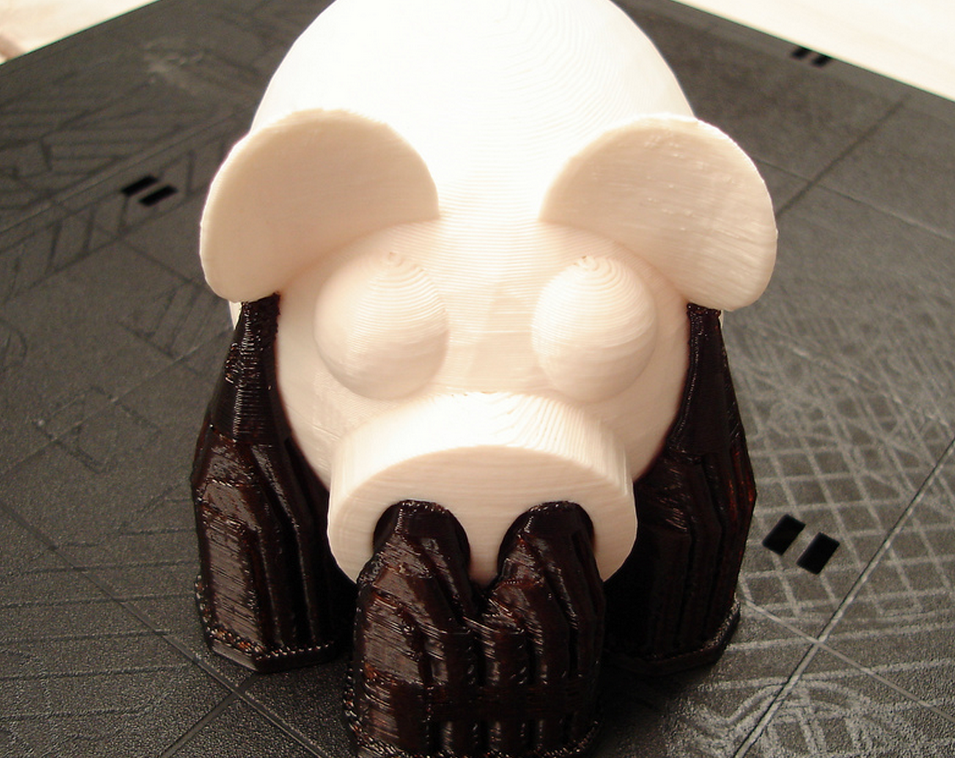
\includegraphics[width=2in]{images/uprint.png}
                \caption{This pig was made on an industrial printer.  Note fine lines and dissolvable support (black).}
                \label{fig:uprint}
        \end{subfigure}
        \begin{subfigure}[b]{0.3\textwidth}
                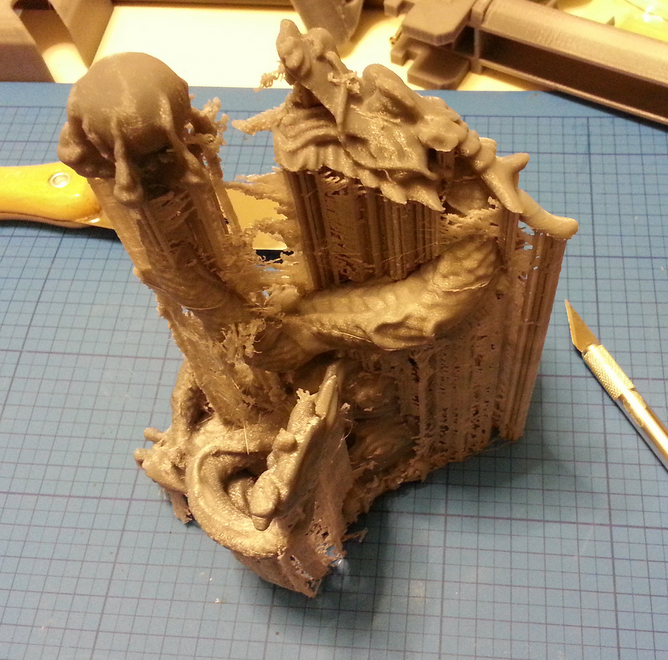
\includegraphics[width=2in]{images/printbefore.png}
                \caption{This Chinese dragon was made on a hobbyist 3D printer.  The rough material is support.}
                \label{fig:makerbot}
        \end{subfigure}
        \begin{subfigure}[b]{0.3\textwidth}
                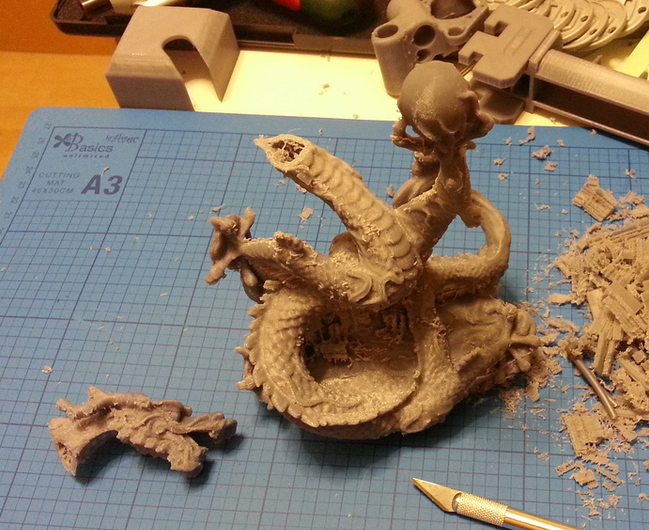
\includegraphics[width=2in]{images/printafter.png}
                \caption{This is the dragon print after support was removed.  The head has broken off.}
                \label{fig:makerbotafter}
        \end{subfigure}
        \caption{Hobbyist and industrial 3D printers have very different abilities.}\label{fig:printers}
\end{figure}


\section{Introduction}
3D printing has become an entrenched part of the prototyping process for professional industrial designers, and thanks to patent expiry it has begun to proliferate as a practice among hobbyists.  However, there are many important differences in the ways that printers are used between these two groups.

The most important practical differences are related to machine specifications.  FDM-style 3D printers (popular among both hobbyists and professionals) work by laying down layers at a time of a typically plastic-like material, melting it out in strands and fusing each layer to the previous one.  This only works if there is something in the layer underneath: in 3D printing culture, this is known as the 45 degree rule.  Overhang angles in an FDM part cannot be greater than 45 degrees without support material underneath.  Here is the difference between hobbyist and professional machines: professional machines offer \emph{two different} materials, one for the model and one for support (see Figure \ref{fig:uprint}).  In this design, the support material is created to dissolve or melt, so that the final model part is simple to extract.  In contrast, hobbyist-level printers are limited to just \emph{one}.  This means that extracting the model from the support material can be a time-consuming process, which is potentially damaging to the model itself (see Figures \ref{fig:makerbot} and \ref{fig:makerbotafter}).

Another crucial difference between the machines used by hobbyists and professionals is their \emph{reliability}.  A professional can typically start a print and walk away, allowing it to run its course.  In contrast, hobbyist machines must be carefully observed until at least two layers have been laid down, to ensure that the print sticks to the bed correctly and that the calibration of the machine is correct.  Even once these layers have been laid, problems such as a tangled material feed or self-destructive vibration can cause a print to fail.  As such, time invested in a print on a hobbyist machine is much more precious, and many hobbyist 3D printers are loath to run extended unsupervised print jobs.

Other differences between professionals and hobbyists are in the types and complexities of models they design, the tools they use for design, and in their uses of the final artifacts.  However, we selected to focus on the support material for our visualization topic.

Several things arise in conversations about support material, including time to print, support material volume, difficulty or time to remove support material, and faces covered in support material.

\subsection{Time to Print}
The time it takes for a part to print on FDM-style machines increases monotonically (but not linearly) with the amount of material required in a print.  The non-linear relationship is due to acceleration settings on most machines, which speed up long, straight lines.  As mentioned, hobbyists prefer not leaving printing models unattended for extended periods of time.

\subsection{Support Material Volume}
Support material from hobbyist-level printers cannot be recycled as yet.  Some support materials, for example PLA which is produced from corn, are biodegradable, however the most popular material--ABS--creates waste that does not degrade easily.  Support material is also not free, and costs a set amount per unit volume used in a print.  Hobbyists are in general sensitive to wasting money and creating waste, so the volume of support material printed is a concern for them.  Irrespective of the orientation of the model, the volume of material used for the model does not change, so this can be disregarded.

\subsection{Support Material Removal}
Removal of support material is an issue for hobbyist machines.  Because support is fabricated of the same material as models, separating support layers from model layers can be challenging.  The main issues that contribute to support material removal time are surface area of model contacted by support material, angle of incidence of support material on model, surfaces affected by support material, connected components of support material, curvature of surface contacted by support material, and accessibility of support material.

\subsubsection{Surface Area}
The surface area of a model contacted by support material is directly proportional to the support removal time.  Larger surface areas in contact with support lead to longer removal times.

\subsubsection{Angle of Incidence}
The angle at which support contacts model affects support removal time.  Support which has a contact of 90 degrees is significantly easier to remove than support contacting at an oblique angle.

\subsubsection{Affected Faces}
Because the support material removal process can be rough, model makers may orient a model in order to keep faces with small details support-free to avoid damaging them.  For example, the face structure of the model in Figure \ref{fig:face} would be made rough by support removal.

\subsubsection{Connected Components}
Support material adheres well to itself, and is easiest to pull off as larger chunks.  The more connected components there are created in support material for a model, the longer it will take to remove because leverage from one component can't be applied to another.

\subsubsection{Curvature}
Model surfaces don't always have smooth and slight curves.  When printing a model like a person's head, quickly-varying curvature over the surface makes material more difficult to remove.  Smooth curves over large areas are easy to pry support from, however detailed peaks and valleys in small spaces are more difficult to extract support from.

\subsubsection{Accessibility}
3D printers have opened up worlds beyond traditional manufacturing processes, and many objects that can be fabricated with a 3D printer cannot be fabricated with any other type of machinery.  Designs can have completely enclosed, freely-moving parts, printed-in-place mechanisms like hinges or chain links, or any of a number of other interesting configurations.  To allow these types of creations to be printed, support material is sometimes very difficult to access from the outside of a model.

We did not have time to focus on all of these metrics, however we have created a visualization tool for 3D designers to explore \emph{time to print, support material volume, surface area, angle of incidence,} and \emph{affected faces}.

\section{Related Work}
There are two main areas of work which we build off for Support Support.  The first is visualization design and sampling over multidimensional spaces.  The second is in actual 3D printing tools.

\subsection{Visualization Design}
In terms of visualization design, there are multiple prior works in the space of multi-dimensional sampling and optimization.

The most crucial works are on evenly sampling the surface of a sphere.  The 6D position of a 3D print is reducible to the three directional dimensions, since location in X, Y on the print bed does not affect print time or support, and, since by increasing Z we only cause more support structure to be created underneath, we can safely assume that Z position will be as close to 0 as possible.

Randomly sampling that 3-dimensional space is a spherical point picking problem.  Spherical point picking has been studied previously by mathematicians.  To pick a random point on the surface of a unit sphere, it is incorrect to select spherical coordinates $\theta$ and $\phi$ from uniform distributions theta in [0,2$\pi$) and $\phi$ in $[0,\pi]$, since the area element $d\Omega=sin\phi d\theta d\phi$ is a function of $\phi$, and hence points picked in this way will be "bunched" near the poles \cite{wolfram}.  In \cite{sphere-point} Marsaglia offers an elegant way of selecting randomly distributed points on the surface of a sphere: in essence, two numbers $x_1$ and $x_2$ are chosen from independent uniform distributions on $(-1, 1)$ and pairs that do not satisfy $x_1^2 + x_2^2 < 1$ are rejected.  Points x, y, and z are then created with $x = 2x_1\sqrt[]{1-x_1^2-x_2^2}$, $y = 2x_2\sqrt[]{1-x_1^2-x_2^2}$, $z = 1 - 2(x_1^2 + x_2^2)$.

We initially built off this work, however with further literature and practical review we realized that in 3D printing it is not actually a sphere that is optimized over!  A 2-dimensional square will do.  Rotation about the z-axis (yaw) does not affect support material usage, accessibility, or any of our other metrics.

Multidimensional sampling and optimizations have been explored in visualization previously, as mentioned.  The foundational work on this was Design Galleries \cite{design-galleries}.  Marks, et al., sampled their multidimensional spaces before a user interacted with their system, generating a projection of the sampled functions into a 2D grid with points where their samples came from.  Users could click on sampled points to see the results of rendering a digital scene with those parameters.  We leverage this technique for the design of our visualization, and we extend their work by focusing also on distributions of several numerical measurements unrelated to the visual look of a generated sample.

\subsection{3D Printing}
There are numerous tools available for free or a fee which assist users with certain tasks in 3D printing.  These tools are mostly focused on offering flexibility for users to customize their prints, rather than comparing different options.

The usual stages a user goes through to 3D print a model are orient, slice, and print.  Some typical examples of interfaces that users use for this are Cura \cite{cura} and Willit 3D Print \cite{willit}.  Cura and Willit are frontends which allow the user to freely rotate their model in space, and which can then call slicers.

Slicers are programs which cut the 3D model into "slices", determine where support is necessary (i.e. where model overhang is greater than 45 degrees), and generate toolpaths through which the printer head will move during the printing process.  They are typically separate from the frontend orientation programs.  Two example slicing engines are Cura Engine \cite{cura-engine} and Skeinforge \cite{skeinforge}.

Designers usually use their orientation frontends to interface with their printers.  They send the slicer-generated GCode instructions to the printer for execution.

Some services, e.g. Shapeways \cite{shapeways} and the aforementioned Willit, offer boolean "will it print" answers.  Users can upload a model and are informed whether it will print by their selected process.  Examples of features which could prevent printability are very thin features (i.e. which are too thin to recreate with the printer's filament) or very large objects (i.e. which do not fit in the printer).  We go beyond this binary yes/no to offer more feedback on a printable objects' properties along particular dimensions.

\subsection{Fabrication and Visualization}
There has been little work in this area of intersection, Jansen, et al., in \cite{jansen-physvis} explored 3D-printed visualizations of bar charts and how their physicality influenced time required and accuracy attained for users to read values, comparing the physical visualizations to digital and AR visualizations.  Our work is focused on generating visualizations about fabrication, rather than visualizations with fabrication.

\begin{figure}
\centering
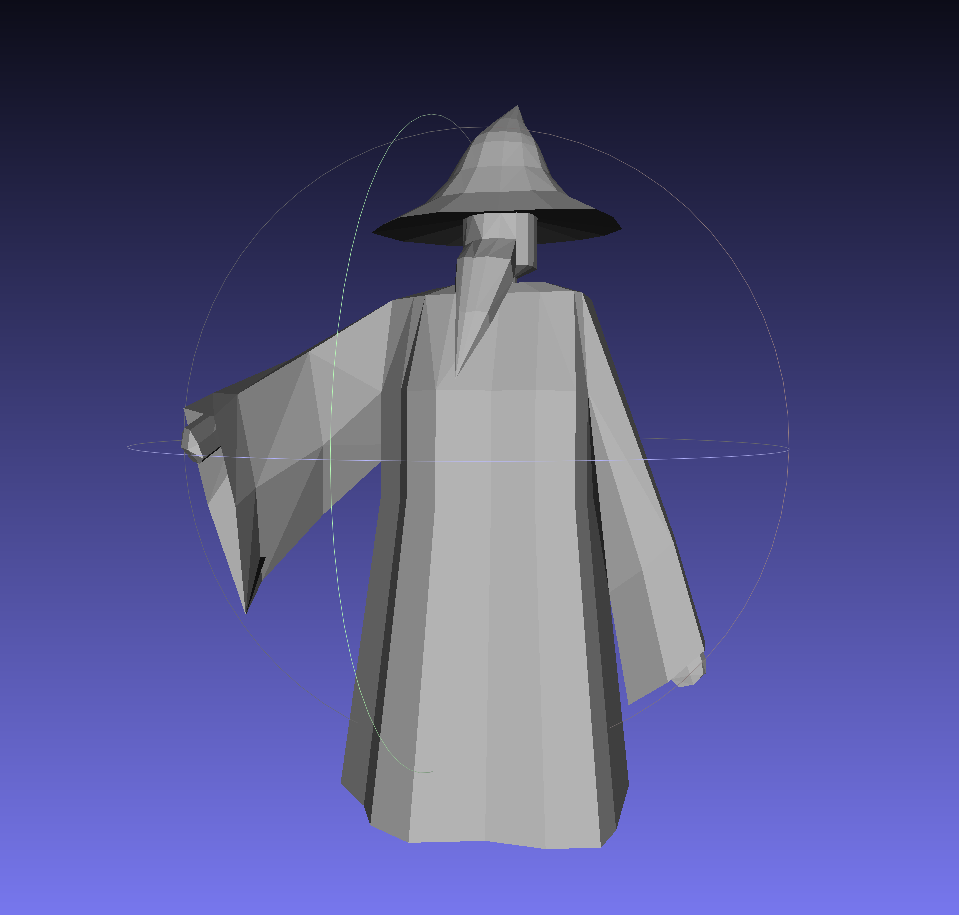
\includegraphics[width=3.25in]{images/wizzard.png}
\caption{Wizzard.stl, a file downloaded from the 3D printing community site Thingiverse.  Notice that there are several greater than 45 degree overhangs in this model, especially around the draping sleeves.}
\label{fig:wizzard}
\end{figure}

\section{Support Supporting a Wizzard}
A novice printer user surfing a 3D printing community website finds a design that she likes created by another user.  She downloads the STL for this file, Wizzard.STL, to her computer.  The designer who uploaded the design did not include instructions about optimal printing orientation, and our user notices (see Figure \ref{fig:wizzard})that there are some parts of the model where the overhangs are definitely more than 45 degrees.  This wizzard has sleeves that drape down below his hands which are totally unconnected to anything.  She can immediately see that she will have to use support material for this print.

Being a novice printer user, she decides to fire up Support Support to help her find the best way to print the Wizzard.  She runs the data generation script, and some time later comes back to her computer to look at the visualization of the data generated.

Through looking at the visualization she can easily view three main aspects of fabrication: support material volume, print time, and surface area of support material contact. For each facet there is a heatmap and a histogram associated, where the x and y axis of the heatmap represent the angle rotation along the x and y axises respectively (see Figure \ref{fig:heatmap}).

\begin{figure}
\centering
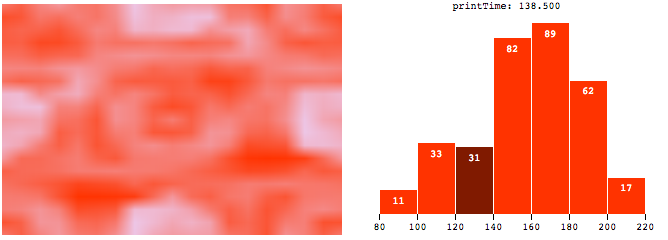
\includegraphics[width=3.25in]{images/heatmap.png}
\caption{The generated heatmap and histogram for print time.  Red is a longer print time (in minutes), and white is a shorter print time.  The Wizzard is rotationally fairly symmetrical, so many rotations give similar results.  Also note that the heatmap wraps around, with the top and bottom edges and left and right edges matching up.}
\label{fig:heatmap}
\end{figure}

She can click on different portions of the heatmaps.  Our user is very interested in environmental topics and the "green-ness" of her print, particularly its waste generation. Thus, she clicks on any of the white portions of the material use heatmap. Upon clicking a point on the heatmap, the wizzard is rotated into the corresponding orientation, and Support Support highlights the histogram bucket which holds that orientation's material use. For this example, the bar would be farthest to the left, since she clicked on a point of very little support material use.

For the selected orientation, our user can also look at the support material angles histogram: this maps out the histogram of connecting angles where these support material contacts the model. She notices that this orientation's angle distribution is stilted towards higher angles.  She knows that support material contacting the model at a 90 degree angle is much more difficult to remove than support material contacting at a 10 degree angle. Therefore, despite her desire to green, she is not feeling particularly gung-ho about having to remove inconvenient support material today. Thus she selects on other light portions on the material use heatmap, and continues to further explore universe of orientations for her Wizzard print.

\begin{figure}
        \centering
        \begin{subfigure}[b]{0.3\textwidth}
                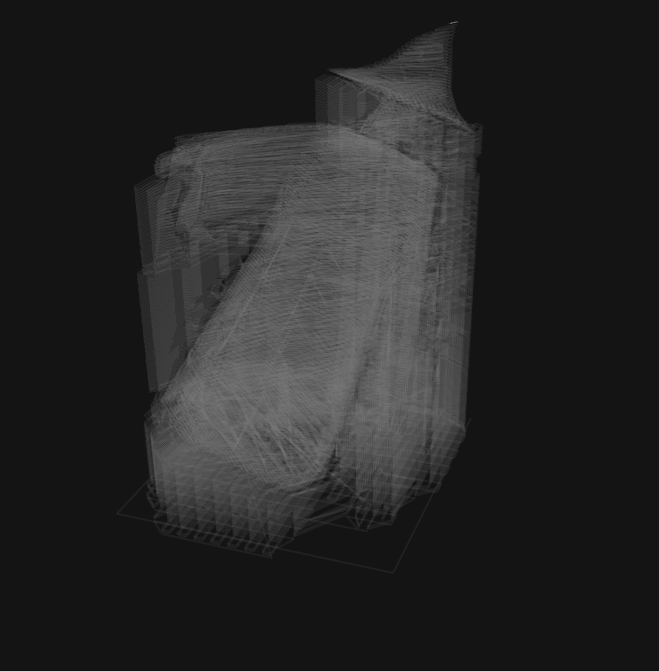
\includegraphics[width=2.75in]{images/wizzard-lotssupport}
                \caption{In this orientation, the wizzard requires lots of support.  Wizzard rotated 20 degrees X, 20 degrees Y.}
                \label{fig:lots}
        \end{subfigure}
        \begin{subfigure}[b]{0.3\textwidth}
                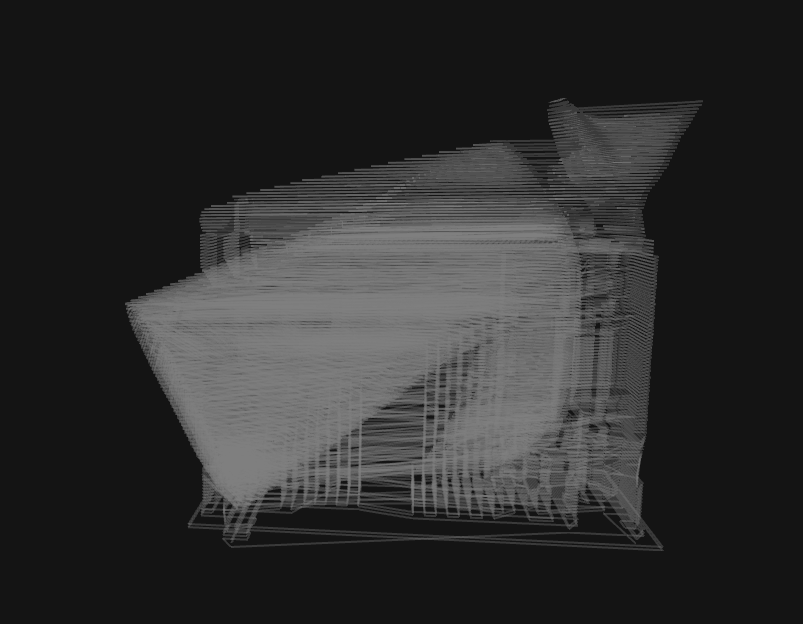
\includegraphics[width=2.75in]{images/wizzard-somesupport}
                \caption{Here, the wizzard requires some support.  Wizzard rotated 60 degrees X, 0 degrees Y.}
                \label{fig:some}
        \end{subfigure}
        \begin{subfigure}[b]{0.3\textwidth}
                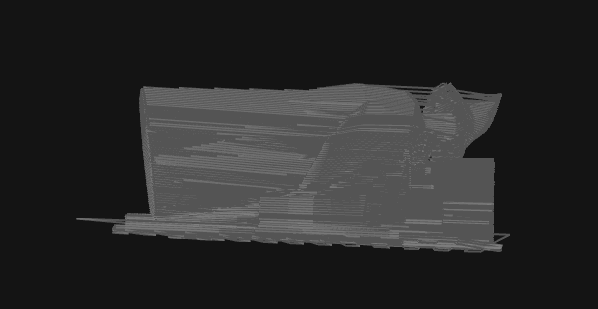
\includegraphics[width=2.75in]{images/wizzard-facesupport}
                \caption{Laid this way, the wizzard has support on his face.  Wizzard rotated 80 degrees X, 120 degrees Y.}
                \label{fig:face}
        \end{subfigure}
        \caption{Depending upon his rotation in X and Y, our wizzard can have lots of support, some support, or support on his face.  Any of these can be considered problems.}\label{fig:rotations}
\end{figure}

\section{Design Decisions}
We wanted to consider the use case described above in our interface design.  See Figure \ref{fig:full} for our final interface.

\begin{figure}
\centering
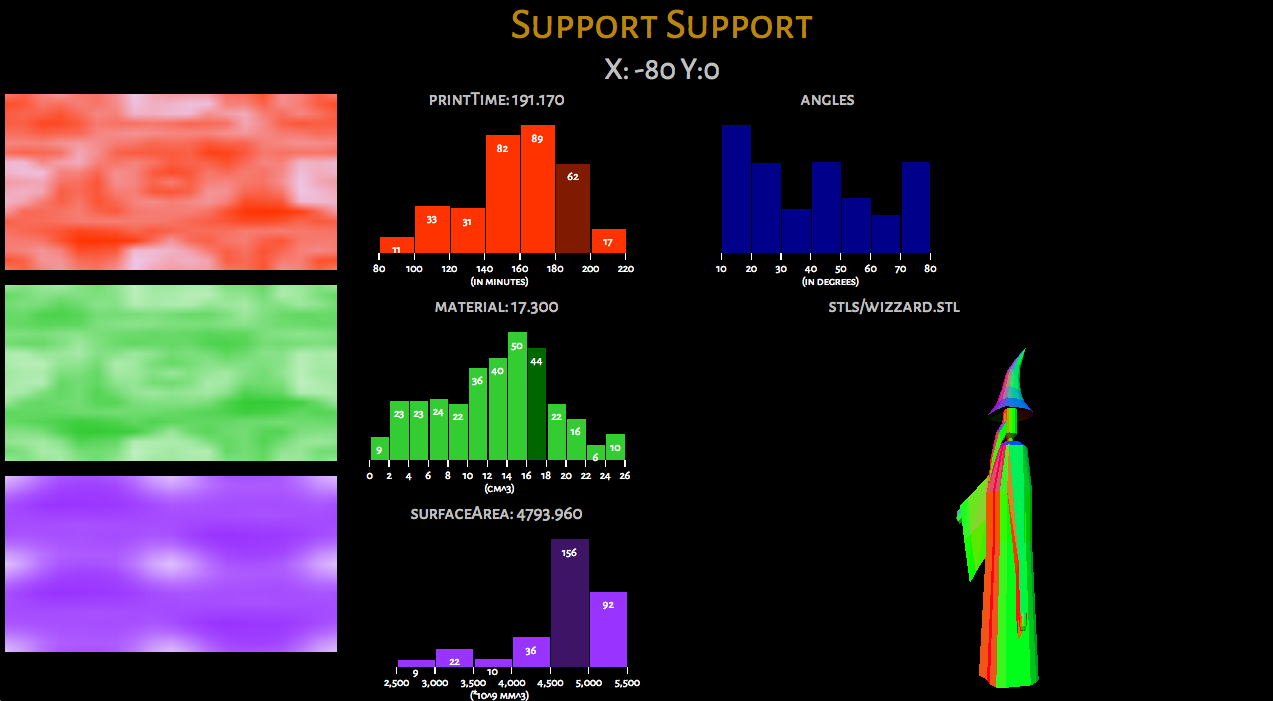
\includegraphics[width=3.25in]{images/fullInterface.png}
\caption{Our final in-browser interface.  Heatmaps and histograms of statistics appear on the left, and the model in the currently-selected orientation appears on the right.  Print time appears in red, support material use in green, and surface area of model contacting support material appears in blue.  The model faces are colored by normal so the user can easily see the shape of the object.}
\label{fig:full}
\end{figure}

The data we generated is of several types.  Our independent variables, X and Y rotation, are quantitative variables that we had to sample (as a continuous dataset would take infinite time to create).  We selected a step size of 20 degrees as we consider this to give a good balance of coverage and time usage.

Our dependent variables--print time, material use, surface area of contact, and surface normals--are also all quantitative variables.  We elected to show a heatmap of how print time, material use, and surface area vary over the XY rotational orientation space.  We also decided to vary this heatmap from white to a specific color (which is different for each variable), with white being the lowest values.  In all cases, a whiter value is better for the user.

We decided to show histograms of the full range of values we found alongside these heatmaps.  The heatmaps give a sense of spatial orientation and smooth variation to the user, while the histograms show her the distribution of values.  Additionally, we highlight the appropriate histogram bucket when the user selects a heatmap point: the smoothly varying color of the heatmaps does not allow the user to easily determine the exact \emph{value} of the dependent variable at the chosen location, nor its relative \emph{goodness} compared to all values sampled.  Displaying this value and highlighting the histogram bar allow the user to determine these facts.

For the STL model we display, we highlight the faces based on their normals.  This technique is available for use in many professional 3D modeling tools, for example Solidworks and Blender, to convey the shapes of objects.

\section{Implementation}
The visualization we implemented is broken down into two parts: data generation and visualization.  Data generation is done offline and ahead of time.  The visualization is visible and available for interaction in-browser.

\subsection{Data Generation}
To create data for our visualization, we randomly sample the space of possible rotations in X and Y.  As mentioned, rotation in Z does not affect any of the statistics we measure.  We create this set of rotations, and then we programmatically rotate the user's STL file and make a copy of it in each rotation.  This collection of STL files is forwarded to the data generation portion of the pipeline.

Data generation is accomplished by logging aggressively during a slicing program's slicing process.  The data we gather are, as mentioned, time to print, support material volume, surface area, angle of incidence, and affected faces.  We used Cura and Skeinforge, both open-source slicing engines, to generate portions of this data.

The types of data that we collect for this visualization are as follows:
\begin{itemize}
\item support material volume
\item time to print
\item surface area of support material contact with model
\item model faces contacted by support material
\item angle of contact of support material on each face
\end{itemize}

All of these data are collected through a combination of added calculation in the slicing programs, extensive logging during the slicing process, and post-slicing log processing with python.

\subsubsection{Rotations}
Rotations are generated using a python script.  Since we identified that rotation in Z did not affect our metrics, we use random selection over two independent distributions on $(-\pi,\pi]$ to select the X and Y rotation.

With the rotations selected, we generate one-time scripts for the programmatic 3D modeling program OpenSCAD.  These scripts are used to call OpenSCAD on the commandline.  This process saves out STL files with the proper rotations of the original.

\subsubsection{Volume and Time}
The support material volume and time to print are both calculated using Skeinforge, which is a pure python slicing program that is no longer actively supported.  We selected it for this portion of the data generation because, though it runs slower than new slicing software, the code was much better commented and easy to work with.

Support material volume is calculated by first slicing the model with no support.  This value, the base material use, is stored.  We then slice the model in all generated orientations and calculate the volume of the total print.  We subtract our stored base material use from the volume of each orientation, giving us the support material use in each orientation.  Note that the volume of material used for the model does not change in different orientations.  Some examples of slicings generated by Skeinforge are shown in Figures \ref{fig:lots} and \ref{fig:some}.

Time to print is calculated using heuristics about the printer's speed moving in XY and Z.  By parsing the generated machine code for the printer, we can sum the execution time over all commands sent to the printer.  This estimated time can be slightly inaccurate; many 3D printers now have hardware acceleration which allows them to print long lines more quickly per distance than short lines. We do not account for this in our data gathering.

\subsubsection{Surface Area, Affected Faces, and Angles}
Our remaining metrics are calculated using Cura, an open-source slicing engine written in C++.  It is more powerful and well-abstracted than Skeinforge, in addition to running faster, so it was ideal for these remaining metrics.

Supported surface area of the model is calculated alongside support.  As the triangles of the STL file are iterated over, we consider only those flagged as needing support.  Using the three vertices (in 3-space) of the triangles, we calculate the area of the triangle ABC as follows:

\begin{enumerate}
\item Find angle between AB and AC, using $AB \cdot AC = |AB||AC|cos\theta$
\item Calculate area using $A = \frac{1}{2}|AB||AC|sin\theta$
\end{enumerate}

We sum over the areas of all supported triangles.  We are also interested in which triangles have support attached to them, so alongside this area calculation, we also log the 3D coordinates of the vertices of all triangles that contact support.

In its usual generation of supports, Cura calculates the angle of the support material's contact with the surface.  It uses this for the purpose of creating accurate machine code where the support material meets the model material's surface.  We simply log these angles as they are calculated and keep a running count of faces found at each orientation; we later take the average of these values.

\subsection{Visualization}
The Support Support visualization is built using three.js \footnote{http://threejs.org} and d3.js \footnote{http://d3js.org}.

\subsubsection{STL Model}
The STL models are rendered using three.js which is a wrapper on top of WebGL. Its takes the ascii STL file and parses it, rendering the STL file in the webview triangle by triangle. Instead of loading up a new STL file everytime the STL file is rotated, we instead rotate the ThreeJS generated model.  The faces of the STL model are colored by their normals, with the red channel being the X portion of the normal, the green channel being the Y portion, and the blue channel being the Z portion.  Normals are calculated using the vertices and their order.

Our plan was to highlight faces that are contacted by support material in a given configuration.  Due to time constraints and unexpected treatment of faces by three.js, we were unable to implement this feature.  However, we are confident that it is possible and plan to implement it as part of our future work.

\subsubsection{Heatmaps and Histograms}
The heatmaps are generated utilizing canvas. Since our data samples the rectangular subspace of degrees at a step of 20 degrees, the heatmap is sparse, requiring us to do bilinear interpolation. We achieve this by interpolating first in X, then in Y to find an estimated measurement value for each pixel.  We map these into colors using d3.js's scale.

The histograms are created using d3.js as well. We added brushing and linking such that clicking on different portions of the heatmap highlights its respective bar on the histogram.

As for the color, we keep the color consistent between the histogram and the heatmap. Time to print is red, support material volume is blue, and total surface area covered is purple.

\section{Evaluation}
Our initial informal user tests with regular users of 3D printers have been very positive.  They all expressed a desire to perform the optimizations supported by Support Support, in particular those users who have only been using the printers for a short time.

We got excellent feature suggestions from them, including the ability to "brush" some faces on the STL where they would prefer not to have support material, as well as providing a series of interface buttons to select the minimum value for each of the measurements we provide (i.e., one button for "minimize print time", one for "minimize surface area", one for "minimize average angle", etc.).  We agree that this would be a valuable option; indeed it would be good to provide users the ability to rank the features that are most important to them and provide a sorted list of possible orientations based on their constraints.

Unfortunately, due to the extreme time requirement for data generation, we showed all our users the wizzard model.  Thus, users also expressed that they would like to see their own models represented in the interface.  We believe this can be accomplished through a system similar to Shapeways, where a user uploads a model and receives an email and link when automatic checks and data generation are complete.

We the authors also have found our visualization to be useful.  We considered our wizzard example.  While the optimal orientation that we generated without looking at statistics is shown in Figure \ref{fig:printed}, the optimal orientation found using our visualization is shown in Figure \ref{fig:printedOptimal}.  We notice that our own orientations are semantically meaningful (in the case of Figure \ref{fig:printed}, the wizzard is on his back).  The data, however, are not tied to semantics, and found a significantly better orientation where the wizzard is at a strange angle and resting on his face and arm.

\begin{figure}
\centering
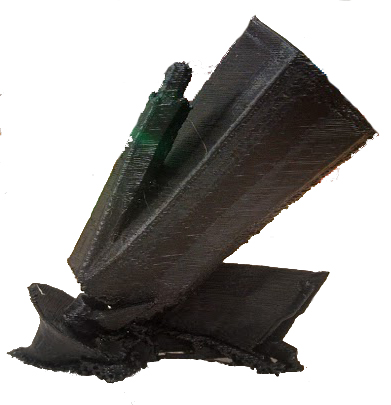
\includegraphics[width=3.5in]{images/printedOptimal.jpg}
\caption{This is the optimal print determined by our interface.  It minimizes material use and print time, and has a very low surface area of support material contact.}
\label{fig:printedOptimal}
\end{figure}

\section{Limitations and Future Work}
There are several considerations of support material and its removal that we do not currently measure, in particular connected components, curvature, and accessibility.  We believe that these measurements are, while not trivial or necessarily computationally efficient, straightforward to determine given sufficient programming time.  Accessibility of support material could be determined with raycasting algorithms.  Curvature and connected components could be tracked by iterating over neighborhoods of each face and comparing measurements.  The time-constrained nature of this project has forced us to focus on the interface and what we believe are the most crucial data.  Additionally, integrating many measurements into an abstract "support removal time" metric would be instructive to novice users who may not understand the relationship between support material angle and support removal time.

As our users stated, another feature that would be very beneficial in future work is brushing and linking with affected faces.  Ideally, a 3D molder would be able to paint faces that should be kept support-free in a print, and use these constraints to narrow the search space of orientations.  Without a sophisticated search index, we were unable to create this function in a way that functioned at interactive speeds.

Our users also pointed out other features that we would like to include in future iterations of Support Support, including minimization buttons.

We believe there is much additional work to be done, both on the visualization and data generation fronts, however Support Support is an initial foray into a previously unexplored space.

\section{Discussion}
Tools for sampling multi-dimensional spaces and visualizations in general have been employed to serve mainly digital needs.  As 3D printers become more ubiquitous and digital design takes to the physical realm, we anticipate that more visualizations will focus on helping novices navigate the complex optimization problems associated with the printing process.  Hopefully some of this is only a stopgap solution.  We anticipate that more multi-material printers will become more affordable to hobbyists, and thereby that the support question will be less difficult.  However, material waste is still a salient issue in even commercial 3D printers with dissolvable supports, as dissolved material is not recoverable.  Even with more sophisticated machines, the fused deposition modeling (FDM) process can still give rise to issues with differing resolution in XY and Z, and also can be subject to shearing at layer interfaces when forces are applied.  We believe that orientation tools to help users explore the tradeoffs for different orientations will evolve with printers, and Support Support is just the start.

\section{Conclusion}
Support Support is a data generation pipeline and visualization designed to save inexperienced designers time in their search to balance material use, printing time, and post-print cleaning time.  We have designed with our own experiences in mind, and with the input of others with 3D printing experience.  There are innumerable features that could be added to a visualization such as this, and additionally it will become more useful as the preprocessing time approaches 0.  A model for creating a better sampling process, i.e. to optimize for one or more user-selected parameters, would obviously make Support Support even more usable in the future.

We are excited to release Support Support into the wild with instructions for users to create their own deployments, and possibly to provide a hosted solution to which users can submit their own models and later see data for them.  We expect that we will get more feedback on it through this process, and plan to continue developing it in our spare time as it serves many of our own needs.

\section{Acknowledgements}
This material is based upon work supported by the National Science Foundation under Grant No. DGE 1106400.  The authors would like to thank the kind users of the Ultimaker forums for their assistance with Cura and data generation.

\balance
\bibliographystyle{acm-sigchi}
\small
\bibliography{references}

\end{document}
